\documentclass[tikz,border=6pt]{standalone}
\usepackage{tikz}
\begin{document}
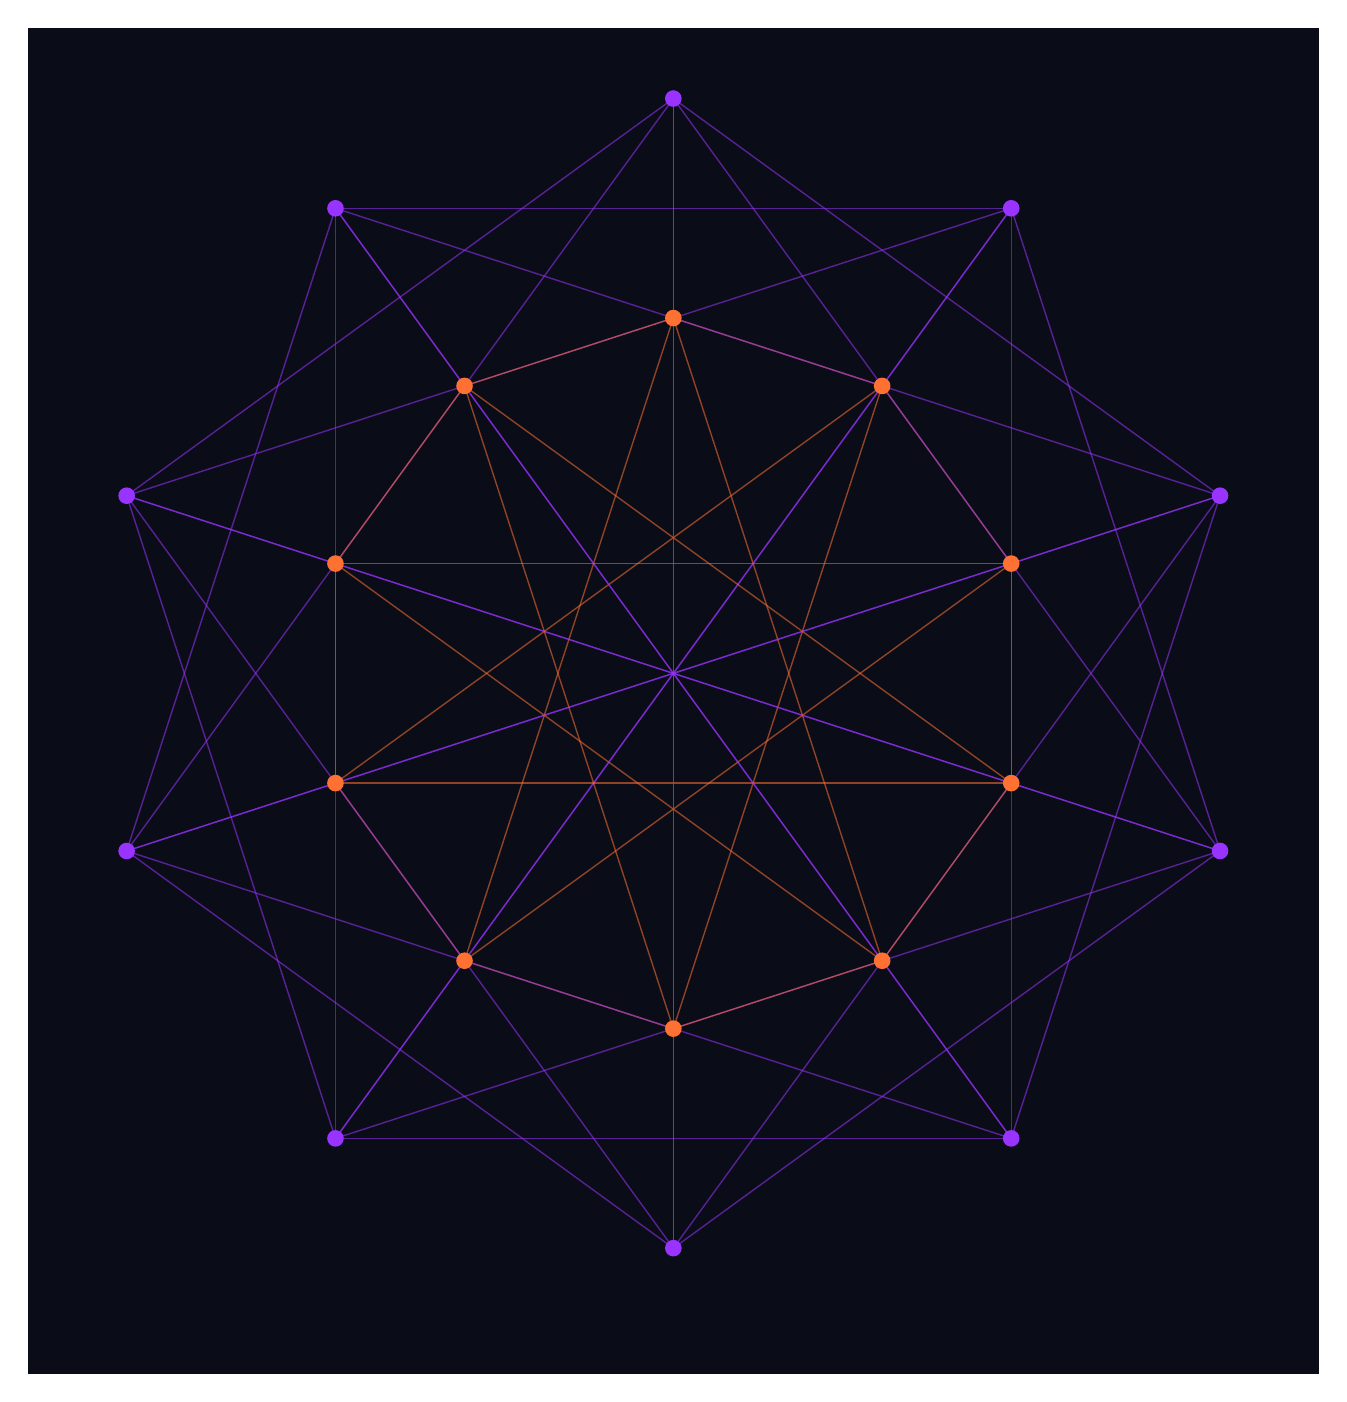
\begin{tikzpicture}
\definecolor{ring0}{rgb}{1.000,0.440,0.200}
\definecolor{ring1}{rgb}{0.600,0.200,1.000}
\definecolor{bg}{rgb}{0.04,0.05,0.09}
\fill[bg] (-8.2,-8.9) rectangle (8.2,8.2);
\draw[ring0,line width=0.5pt,opacity=0.55] (2.652,3.650)--(0.000,-4.512);
\draw[ring1,line width=0.5pt,opacity=0.55] (2.652,3.650)--(-4.291,-5.906);
\draw[ring0,line width=0.5pt,opacity=0.55] (2.652,3.650)--(0.000,4.512);
\draw[ring0,line width=0.5pt,opacity=0.55] (2.652,3.650)--(-4.291,-1.394);
\draw[ring1,line width=0.5pt,opacity=0.55] (2.652,3.650)--(4.291,5.906);
\draw[ring0,line width=0.5pt,opacity=0.55] (2.652,3.650)--(4.291,1.394);
\draw[ring1,line width=0.5pt,opacity=0.55] (6.943,2.256)--(4.291,-5.906);
\draw[ring1,line width=0.5pt,opacity=0.55] (6.943,2.256)--(-0.000,-7.300);
\draw[ring1,line width=0.5pt,opacity=0.55] (6.943,2.256)--(-4.291,5.906);
\draw[ring1,line width=0.5pt,opacity=0.55] (6.943,2.256)--(-4.291,-1.394);
\draw[ring1,line width=0.5pt,opacity=0.55] (6.943,2.256)--(0.000,7.300);
\draw[ring1,line width=0.5pt,opacity=0.55] (6.943,2.256)--(4.291,1.394);
\draw[ring1,line width=0.5pt,opacity=0.55] (6.943,-2.256)--(4.291,-1.394);
\draw[ring1,line width=0.5pt,opacity=0.55] (6.943,-2.256)--(-0.000,-7.300);
\draw[ring1,line width=0.5pt,opacity=0.55] (6.943,-2.256)--(-4.291,1.394);
\draw[ring1,line width=0.5pt,opacity=0.55] (6.943,-2.256)--(-4.291,-5.906);
\draw[ring1,line width=0.5pt,opacity=0.55] (6.943,-2.256)--(0.000,7.300);
\draw[ring1,line width=0.5pt,opacity=0.55] (6.943,-2.256)--(4.291,5.906);
\draw[ring0,line width=0.5pt,opacity=0.55] (2.652,-3.650)--(4.291,-1.394);
\draw[ring1,line width=0.5pt,opacity=0.55] (2.652,-3.650)--(4.291,-5.906);
\draw[ring0,line width=0.5pt,opacity=0.55] (2.652,-3.650)--(-4.291,1.394);
\draw[ring0,line width=0.5pt,opacity=0.55] (2.652,-3.650)--(0.000,-4.512);
\draw[ring1,line width=0.5pt,opacity=0.55] (2.652,-3.650)--(-4.291,5.906);
\draw[ring0,line width=0.5pt,opacity=0.55] (2.652,-3.650)--(0.000,4.512);
\draw[ring0,line width=0.5pt,opacity=0.55] (-2.652,-3.650)--(0.000,-4.512);
\draw[ring1,line width=0.5pt,opacity=0.55] (-2.652,-3.650)--(-4.291,-5.906);
\draw[ring0,line width=0.5pt,opacity=0.55] (-2.652,-3.650)--(0.000,4.512);
\draw[ring0,line width=0.5pt,opacity=0.55] (-2.652,-3.650)--(-4.291,-1.394);
\draw[ring1,line width=0.5pt,opacity=0.55] (-2.652,-3.650)--(4.291,5.906);
\draw[ring0,line width=0.5pt,opacity=0.55] (-2.652,-3.650)--(4.291,1.394);
\draw[ring1,line width=0.5pt,opacity=0.55] (4.291,-1.394)--(-6.943,2.256);
\draw[ring0,line width=0.5pt,opacity=0.55] (4.291,-1.394)--(-4.291,-1.394);
\draw[ring0,line width=0.5pt,opacity=0.55] (4.291,-1.394)--(-2.652,3.650);
\draw[ring0,line width=0.5pt,opacity=0.55] (4.291,-1.394)--(4.291,1.394);
\draw[ring1,line width=0.5pt,opacity=0.55] (4.291,-5.906)--(-6.943,-2.256);
\draw[ring1,line width=0.5pt,opacity=0.55] (4.291,-5.906)--(-4.291,-5.906);
\draw[ring1,line width=0.5pt,opacity=0.55] (4.291,-5.906)--(-2.652,3.650);
\draw[ring1,line width=0.5pt,opacity=0.55] (4.291,-5.906)--(4.291,5.906);
\draw[ring1,line width=0.5pt,opacity=0.55] (-0.000,-7.300)--(-6.943,-2.256);
\draw[ring1,line width=0.5pt,opacity=0.55] (-0.000,-7.300)--(0.000,-4.512);
\draw[ring1,line width=0.5pt,opacity=0.55] (-0.000,-7.300)--(-6.943,2.256);
\draw[ring1,line width=0.5pt,opacity=0.55] (-0.000,-7.300)--(0.000,4.512);
\draw[ring1,line width=0.5pt,opacity=0.55] (-6.943,-2.256)--(-4.291,5.906);
\draw[ring1,line width=0.5pt,opacity=0.55] (-6.943,-2.256)--(-4.291,-1.394);
\draw[ring1,line width=0.5pt,opacity=0.55] (-6.943,-2.256)--(0.000,7.300);
\draw[ring1,line width=0.5pt,opacity=0.55] (-6.943,-2.256)--(4.291,1.394);
\draw[ring1,line width=0.5pt,opacity=0.55] (-4.291,1.394)--(-6.943,2.256);
\draw[ring0,line width=0.5pt,opacity=0.55] (-4.291,1.394)--(-4.291,-1.394);
\draw[ring0,line width=0.5pt,opacity=0.55] (-4.291,1.394)--(-2.652,3.650);
\draw[ring0,line width=0.5pt,opacity=0.55] (-4.291,1.394)--(4.291,1.394);
\draw[ring0,line width=0.5pt,opacity=0.55] (0.000,-4.512)--(-2.652,3.650);
\draw[ring1,line width=0.5pt,opacity=0.55] (0.000,-4.512)--(0.000,7.300);
\draw[ring1,line width=0.5pt,opacity=0.55] (-4.291,-5.906)--(-6.943,2.256);
\draw[ring1,line width=0.5pt,opacity=0.55] (-4.291,-5.906)--(-4.291,5.906);
\draw[ring1,line width=0.5pt,opacity=0.55] (-6.943,2.256)--(0.000,7.300);
\draw[ring1,line width=0.5pt,opacity=0.55] (-6.943,2.256)--(4.291,5.906);
\draw[ring1,line width=0.5pt,opacity=0.55] (-4.291,5.906)--(-2.652,3.650);
\draw[ring1,line width=0.5pt,opacity=0.55] (-4.291,5.906)--(4.291,5.906);
\draw[ring0,line width=0.5pt,opacity=0.55] (0.000,4.512)--(-2.652,3.650);
\draw[ring1,line width=0.5pt,opacity=0.55] (0.000,4.512)--(0.000,7.300);
\fill[ring0] (2.652,3.650) circle (3.0pt);
\fill[ring1] (6.943,2.256) circle (3.0pt);
\fill[ring1] (6.943,-2.256) circle (3.0pt);
\fill[ring0] (2.652,-3.650) circle (3.0pt);
\fill[ring0] (-2.652,-3.650) circle (3.0pt);
\fill[ring0] (4.291,-1.394) circle (3.0pt);
\fill[ring1] (4.291,-5.906) circle (3.0pt);
\fill[ring1] (-0.000,-7.300) circle (3.0pt);
\fill[ring1] (-6.943,-2.256) circle (3.0pt);
\fill[ring0] (-4.291,1.394) circle (3.0pt);
\fill[ring0] (0.000,-4.512) circle (3.0pt);
\fill[ring1] (-4.291,-5.906) circle (3.0pt);
\fill[ring1] (-6.943,2.256) circle (3.0pt);
\fill[ring1] (-4.291,5.906) circle (3.0pt);
\fill[ring0] (0.000,4.512) circle (3.0pt);
\fill[ring0] (-4.291,-1.394) circle (3.0pt);
\fill[ring0] (-2.652,3.650) circle (3.0pt);
\fill[ring1] (0.000,7.300) circle (3.0pt);
\fill[ring1] (4.291,5.906) circle (3.0pt);
\fill[ring0] (4.291,1.394) circle (3.0pt);
\end{tikzpicture}
\end{document}